\documentclass[paper=letter, fontsize=12pt]{article}
\usepackage{geometry}
\geometry{margin=1in}
\usepackage{graphicx}
\graphicspath{{images/}}
\usepackage{amssymb}
\usepackage{enumitem}

%opening
\title{Compsci 571 HW2}
\author{Yilin Gao (yg95)}

\begin{document}

\maketitle
\section{Classifier for Basketball Courts}

\begin{enumerate}[label=(\alph*)]
	\item When running Perceptron algorithm on the dataset, it takes 7 iterations (updates) to converge. The decision boundary is $f(x_1, x_2) = -1.05 * x_1 + 1.1 * x_2$. Because after it converges, all training points are correctly classified, the error rate is 0.
	
	Assume another linear classifier that goes through origin and achieves the same training error rate (0) as the perceptron classifier is $f(x_1, x_2) = w_1 * x_1 + w_2 * x_2$. Set $f(x_1, x_2) = 0$, we get the slope of the boundary is $-\frac{w_1}{w_2}$. From the plot of training data, we know that the boundary should go above point $[0.85, 0.80]$, and go below point $[0.85, 0.95]$. So $\frac{0.80}{0.85} < -\frac{w_1}{w_2} < \frac{0.95}{0.85}$. If we set $w_2 = 1.1$ as the perceptron boundary, we get $-1.229 < w_1 < -1.035$.
	
	The plot of observed data, the perceptron decision boundary (the light blue line), and all other linear boundaries that achieve the same training error (the yellow area) is:
	
	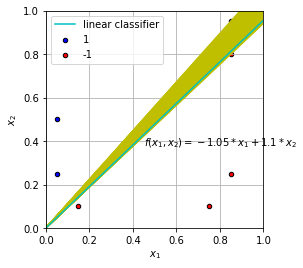
\includegraphics[scale=0.6]{q1a.png}
	
	\item The fully-grown decision tree using Gini index as splitting criterion on the observed data is:
	
	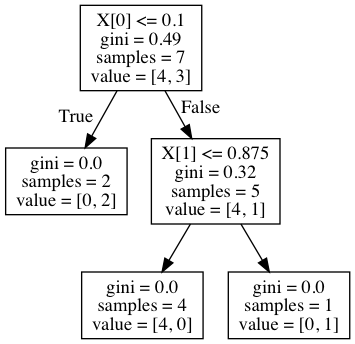
\includegraphics[scale=0.6]{q1b_tree.png}
	
	Because all training points are correctly classified by this tree, its training error is 0.
	
	Assume another decision tree with same training error (0) splits on the same feature order but different splitting threshold ($v_1$ for $x_1$ and $v_2$ for $x_2$). Then the threshold of the first split on $x_1$ should be able to separate points $[0.05, 0.25], [0.05, 0.5]$ (+1) with $[0.15, 0.1]$ (-1). So $v_1$ should be $\in (0.05, 0.15)$. The threshold of the second split on $x_2$ should be able to separate points $[0.85, 0.8]$ (-1) with $[0.85, 0.95]$ (+1). So $v_2$ should be $\in (0.8, 0.95)$.
	
	The plot of observed data, and the calculated decision boundary is:
	
	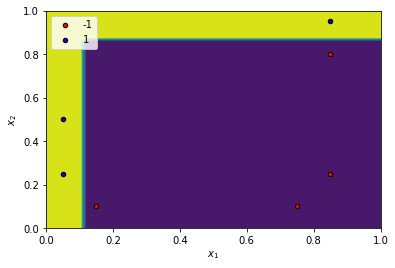
\includegraphics[scale=0.6]{q1b1.png}
	
	The plot of observed data, the calculated decision boundary, and all other decision boundaries that achieve the same training area (the red area) is:
	
	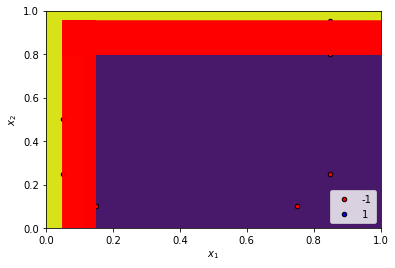
\includegraphics[scale=0.6]{q1b2.png}
	
	\item 
	
	\item 
	
	\item 
	
	\item 
	
	\item 
	
	\item 
	
\end{enumerate}

\section{Variable Importance for Trees and Random Forest}

\begin{enumerate}[label=(\alph*)]
	\item 
	\begin{enumerate}[label=(\roman*)]
		\item 
		The decision stump based on the best split is:
		
		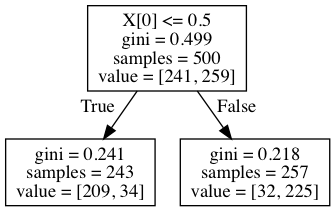
\includegraphics[scale=0.6]{tree_best_split.png}
		
		The decision stump based on the best surrogate split is:
		
		%TODO
		
		\item 
		
		\item 
		The mean least-squares error of predictions on the test data of the decision stump based on the best split is 10.
		
		% TODO
		The mean least-squares error of predictions on the test data of the decision stump based on the best split is 
	\end{enumerate}

	\item 
	\begin{enumerate}[label=(\roman*)]
		\item 
		
		\item 
		
		\item 
	\end{enumerate}

	\item 
	\begin{enumerate}[label=(\roman*)]
		\item 
		
		\item
	\end{enumerate}
\end{enumerate}
\end{document}
